\documentclass[polish,12pt,a4paper]{extarticle}
\usepackage[T1]{fontenc}

\usepackage[top=2.5cm,bottom=2cm,left=2cm,right=2cm]{geometry}
\usepackage{xcolor}

\usepackage{placeins}  % in the preamble
\usepackage{babel}
\usepackage{titling}
\usepackage{lastpage}
\usepackage{amsmath}
\usepackage{amssymb}
\usepackage{stmaryrd}
\usepackage{fancyhdr}
\usepackage[bookmarks=false]{hyperref}
\usepackage{algorithm2e}
\usepackage{mathtools}
\usepackage{xcolor}
%\usepackage{overarrows}
\pagestyle{fancy}

\usepackage{tikz}
\usetikzlibrary{angles,quotes}

\title{Miniprojekt 2}
\author{Jakub Wieliczko}

\fancyhead[l]{MPUM}
\fancyhead[c]{\textbf{\thetitle}}
\fancyhead[r]{\theauthor}
\fancyfoot[c]{\begin{NoHyper}\thepage/\pageref{LastPage}\end{NoHyper}}

\newcommand{\inident}{\hspace{1.25em}}

% Algo stuff
\newcommand\mycommfont[1]{\ttfamily\textcolor{gray}{#1}}
\SetCommentSty{mycommfont}
\newcommand\Field[2]{\textbf{Field} $#1$: \texttt{#2}\;}
\newcommand\Method[3]{
	\SetKwFunction{Fn#1#2}{#1.#2}
	\SetKwFunction{FnLocal#1#2}{#2}
	\MethodImpl{\textnormal{\texttt{#2}(#3)}}
}
\newcommand\Struct[1]{
	\SetKwFunction{St#1}{#1}
	\StructImpl{\textnormal{\texttt{#1}}}
}

\newcommand\initalgorithm{
	\SetAlgoLined
	\DontPrintSemicolon
	\SetKwProg{Fn}{function}{:}{end}
	\SetKwProg{StructImpl}{struct}{:}{end}
	\SetKwProg{MethodImpl}{method}{:}{end}
}

% Math Stuff
\newcommand\Nat{\mathbb{N}}
\newcommand\Primes{\mathbb{P}}
\newcommand\eqqm[0]{\stackrel{?}{=}}
\renewcommand\lor{\,\vee\,}
\renewcommand\land{\,\wedge\,}
\newcommand\lxor[0]{\,\veebar\,}
\newcommand\union[0]{\cup}
\newcommand\isect[0]{\cap}
\newcommand\Union[0]{\bigcup}
\newcommand\Isect[0]{\bigcap}
\newcommand\nil[0]{\emptyset}
\renewcommand\geq{\geqslant}
\renewcommand\leq{\leqslant}
\newcommand\eqs[1]{\stackrel{#1}{=}}
\newcommand\impliesqm[0]{\stackrel{?}{\implies}}
\newcommand\QED[0]{\hfill$\blacksquare$}

\newcommand\set[1]{\left\{#1\right\}}
\newcommand\card[1]{\left|#1\right|}
\newcommand\cset[1]{\card{\set{#1}}}
\DeclarePairedDelimiter{\floor}{\lfloor}{\rfloor}
\DeclarePairedDelimiter{\ceil}{\lceil}{\rceil}

\newcommand{\stirC}[2]{\genfrac{[}{]}{0pt}{}{#1}{#2}}
\newcommand{\stirP}[2]{\genfrac{\{}{\}}{0pt}{}{#1}{#2}}


%\NewOverArrowCommand{image}{}
%\NewOverArrowCommand{coimage}{
%	end=\leftarrow
%}

\newcommand\stdarr[0]{\rightarrow}
\newcommand\injarr[0]{\hookrightarrow}
\newcommand\surarr[0]{\rightarrow\mathrel{\mspace{-15mu}}\rightarrow}
\newcommand\bijarr[0]{\hookrightarrow\mathrel{\mspace{-15mu}\rightarrow}}


\begin{document}


\begin{abstract}
    W poniższym dokumencie przedstawiam wnioski wyciągnięte podczas pisania projektu dot. klasyfikacji z Metod Probabilistycznych w Uczeniu Maszynowym. Celem projektu jest porównanie dwóch algorytmów, naiwnego klasyfikatora bayesowskiego oraz algorytmu regresji logistycznej przy problemie klasyfikacji.
\end{abstract}

\section*{Przygotowanie danych}
Na wejściu otrzymujemy zbiór danych postaci $D = \{(x^{(i)}_1, x^{(i)}_2, \dots, x^{(i)}_9, y^{(i)}): i = 1,2,\dots, m\}$, zatem mamy $9$ niezależnych cech opisujących badanie oraz informację, czy badany rak jest łagodny $(y = 2)$, czy złośliwy $(y = 4)$. Dla ułatwienia będę oznaczał $y = 2$ jako klasę $0$, zaś $y = 4$ jako klasę $1$ W celu podziału tych danych na zbiory treningowy i testowy, dzielę $D$ na $D_0$ i $D_1$ dla danych należących do klas odpowiednio $0$ i $1$, następnie dzielę obydwa zbiory w proporcji $2 : 1$ i łącząc te części tworzę zbiór treningowy $S$ i testowy $T$. W ten sposób losowo wybrana dana z $S$ ma takie same prawdopodobieństwo bycia w klasie $0$, co losowo wybrana dana z $T$. \bigskip \\
Na potrzeby projektu zauważyłem, że każda z cech jest pewną liczbą całkowitą ze zbioru $\{1, 2, \dots, 10\}$. W związku z tym potraktowałem te cechy jako zmienne dyskretne, więc nie stosuję w tym przypadku standaryzacji danych. Przy \textbf{naiwnym klasyfikatorze bayesowskim} standaryzacja danych i tak nie miałaby sensu, a dla \textbf{regresji logistycznej} zakresy tych danych są na tyle małe, że przy liczeniu gradientu nie miało to wpływu na dobranie współczynnika \texttt{learning rate}, czy nie utrudnia wyboru hiperparametru $\lambda$ przy regularyzacji.

\section*{Wstępna analiza danych}



\section*{Regresja logistyczna}
Na potrzeby tego projektu zaimplementowałem regresję logistyczną używając do tego klayscznego algorytmu spadku wzdłuż gradientu. Nie zdecydowałem się na żadne optymalizacje, np. \textbf{mini$-$batch}, gdyż model trenował się względnie bardzo szybko: dla $n = 15000$ iteracji (dla tylu epok wyniki już były satysfakcjonujące), na pełnym zbiorze treningowym przebieg algorytmu zajmował ok. $5$ sekund

\section*{Naiwny klasyfikator Bayesowski}

Ciekawą rzeczą, którą zauważyłem analizując proces trenowania naiwnego klasyfikatora bayesowskiego, było to że gdy używałem więcej niż $12.5\%$ zbioru treningowego to im więcej miał danych, tym bardziej pewne decyzje na zbiorze testowym podejmował. Zatem zdecydowaną część wyników szacował albo na $0.00\%$, albo na $99.99\%$ (decyzje były \textit{troszeczkę} bardziej zrównoważone gdy użyłem \texttt{log-prawdopodobieństwa}, ale odpowiedzi nadal były, delikatnie rzecz ujmując, \textbf{stanowcze}).

\section*{Wyniki}
Miarą, której używam do oceny mojego klasyfikatora jest miara $F_1$, gdyż zależy mi obecnie na modelu który zarówno wykrywa jak najwięcej przypadków i przy okazji unika fałszywych alarmów. \begin{center}
$F_1(\mathrm{precision}, \mathrm{sensitivity}) = \frac{2 \cdot \mathrm{precision} \cdot \mathrm{sensitivity}}{\mathrm{precision} + \mathrm{sensitivity}}$
\end{center}
Pytanie na które chciałbym odpowiedzieć, to ile danych wystarczy żeby satysfakcjonująco wytrenować klasyfikator. W tym celu wytrenowałem obydwa modele na różnych frakcjach zbioru treningowego, a wyniki znajdują się poniżej.
\begin{figure}[h!]
    \centering
    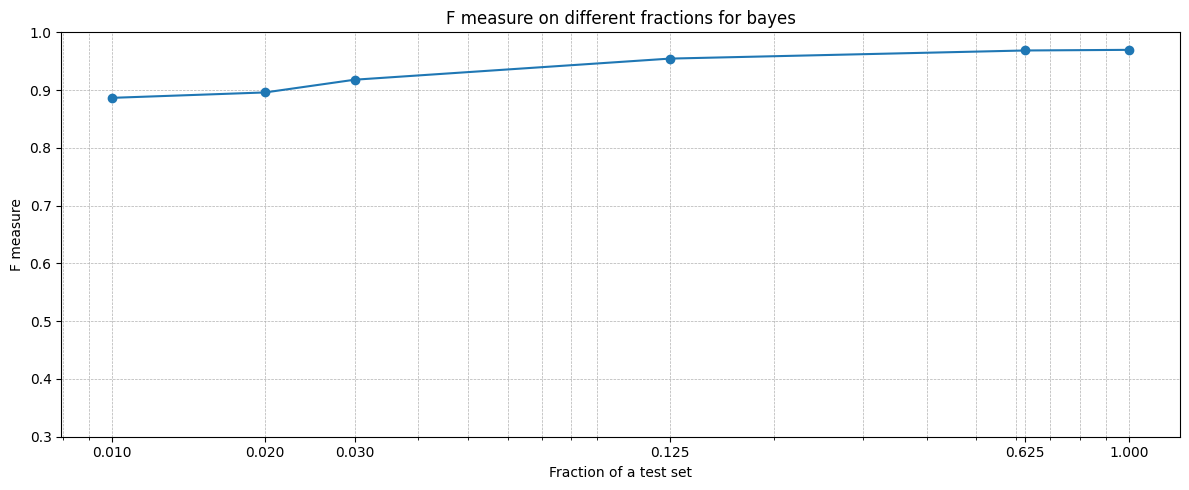
\includegraphics[width=0.85\textwidth]{img/bayes_frac_better.png}
    \caption{Miara $F_1$ dla frakcji przy uczeniu naiwnego klasyfikatora Bayesowskiego}
\end{figure} \\
\begin{figure}[h!]
    \centering
    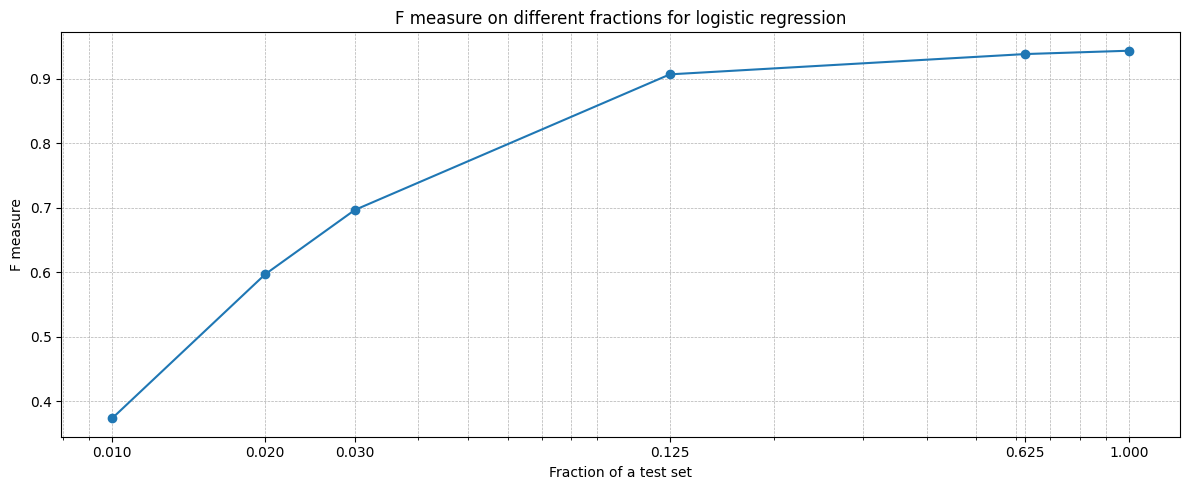
\includegraphics[width=0.85\textwidth]{img/logistic_frac.png}
    \caption{Miara $F_1$ dla frakcji przy uczeniu algorytmem regresji logistycznej}
\end{figure} \\
Od początku widzimy bardzo dużą różnicę. Otóż, gdy popatrzymy na skalę miary $F_1$, naiwny klasyfikator bayesowski od początku radzi sobie dużo lepiej, przy czym już $1\%$ zbioru treningowego pozwala mu na nauczenie się danych na tyle dobrze, żeby otrzymywać średnio miarę $0.89$. Jest to wynik do którego regresja logistyczna zbliża się dopiero przy $12.5\%$ zbioru treningowego, a nasz klasyfikator Bayesowski otrzymuje już miary rzędu $0.96$
\end{document}
